\chapter{Monitoring with \cmd{fxmenet-top}}
\label{ch:top}

\cmd{fxmenet-top} is a terminal program that shows what a server is doing, in
the manner of \cmd{top}. It runs on Linux, macOS and Windows 10 or later,
in any terminal that understands ANSI escape sequences. It connects to the
server's control port as a monitor: it opens no session and never touches
the audio, so it can be started and stopped at will.

\section{Starting it}

\begin{lstlisting}
fxmenet-top                      # the server on this machine
fxmenet-top 192.168.1.20         # a server elsewhere (port 54322)
fxmenet-top studio.local:54322   # with a port
fxmenet-top --once               # print one frame without colours, and exit
fxmenet-top --find               # list the servers on the local network
\end{lstlisting}

If the server stops, \cmd{fxmenet-top} says so and reconnects when it
returns. To disable colours, set the environment variable \cmd{NO_COLOR}.

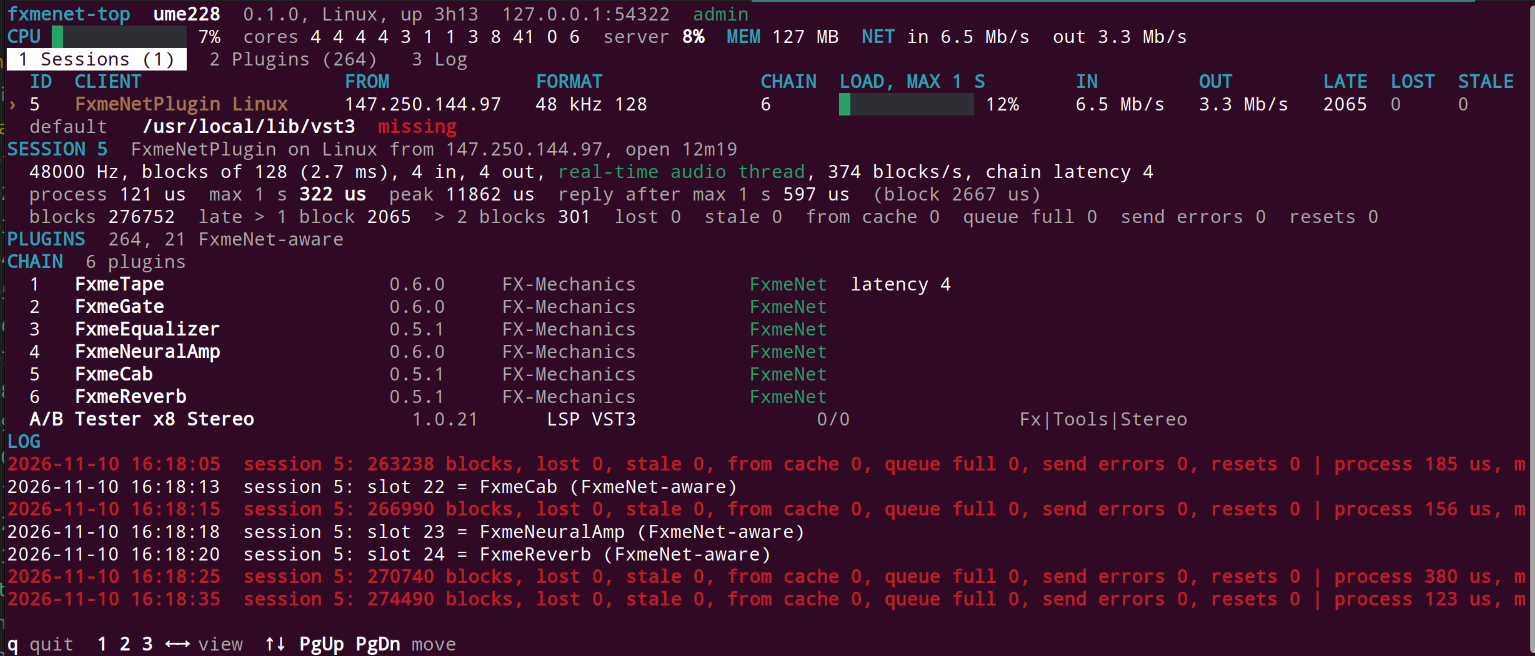
\includegraphics[width=\textwidth]{../img/fxme-net-top.png}


\section{The header}

Two lines are always visible. The first gives the server's name, version,
system and uptime, the address, and whether you may change the plugin folders
(\emph{admin}) or only watch (\emph{read only}). The second gives:

\begin{itemize}
  \item \textbf{CPU}: the machine's total use, each core, and the server
    process's use (100\,\% is one core fully used, as in \cmd{top}). Windows
    does not give the per-core figures.
  \item \textbf{MEM}: the server process's memory.
  \item \textbf{NET}: the audio traffic received and sent.
\end{itemize}

Below them, three views are selected with \key{1}, \key{2} and \key{3} (or the
left and right arrows).

\section{Sessions}

\key{1}. One line per client session: its name and system, its address, the
format (sample rate and block size), the number of plugins, a bar for the
load, the traffic, and the counts of late, lost and stale blocks. The load
bar compares the worst processing time of the last second with the block's
duration: green is comfortable, yellow is getting tight, red means the
server is close to missing deadlines. A count that has just moved turns red
for ten seconds.

Choose a session with the up and down arrows. Under the list, the details
show the format, whether the audio thread has real-time priority, the
processing times, all the counters, and the session's chain with each
plugin's version, vendor and latency. The latest log lines fill the rest of
the screen.

\section{Plugins and folders}

\key{2}. The folders the server searches (default, saved, and given on the
command line), with missing ones marked; the progress of the scan in
progress; and the plugins found, sorted by name. Press \key{/} to filter
them, as in the plugin's own list; \key{Esc} clears the filter.

When you are allowed to (\emph{admin}), these keys change the folders:

\begin{longtable}{@{}p{0.2\textwidth}p{0.74\textwidth}@{}}
\toprule
\textbf{Key} & \textbf{Action}\\
\midrule
\endhead
\key{a} & Add a folder (type an absolute path on the server, then \key{Return}).\\
\key{d} & Remove the selected saved folder.\\
\key{x} & Turn the default VST3 folders on or off.\\
\key{r} & Rescan: new or changed plugins only.\\
\key{R} & Full rescan, ignoring the cache.\\
\key{Tab} & Move between the list of folders and the list of plugins.\\
\bottomrule
\end{longtable}

The scan runs in the background and its progress appears at once. Folders
you add are kept by the server for its next runs.

\section{Log}

\key{3}. The server's log, with the latest lines at the bottom. Scroll with
the arrows, \key{PgUp} and \key{PgDn}; \key{End} follows the newest line again.
Lines that contain \emph{error}, \emph{warning} or \emph{skipped} are red.
\key{/} filters the lines.

\section{Keys}

\begin{longtable}{@{}p{0.28\textwidth}p{0.66\textwidth}@{}}
\toprule
\textbf{Key} & \textbf{Action}\\
\midrule
\endhead
\key{1} \key{2} \key{3} or arrows & Choose the view.\\
\key{Up} \key{Down} \key{PgUp} \key{PgDn} & Move in the list.\\
\key{Home} \key{End} & First or last entry (in the log, the newest).\\
\key{/} & Filter the plugins or the log.\\
\key{Esc} & Clear the filter, or cancel typing.\\
\key{q} & Quit.\\
\bottomrule
\end{longtable}
